\documentclass[a4paper, 12pt]{article}

\usepackage{graphicx}
\usepackage{hyperref}
\usepackage{geometry}
\usepackage{times}
\usepackage{marvosym}
\usepackage{amsmath}
\usepackage{tocloft}
\usepackage{changepage}
\usepackage{multirow}
\usepackage{array}

\geometry{left=2.5cm}
\geometry{right=2.5cm}
\geometry{top=2.5cm}
\geometry{left=3.5cm}
\renewcommand{\baselinestretch}{1.5} 
% \usepackage[utf8]{inputenc}
\graphicspath{ {./images/} }
\usepackage[slovak]{babel}
\hypersetup{
    colorlinks=true,
    linkcolor=black,
    urlcolor=cyan
}


% пустая страница
\newcommand{\emptypage}{

  \newpage
  \thispagestyle{empty}
  \begin{center}
  \end{center}
}

% bold h1
\newcommand{\heading}[1]{\textbf{\Large{ #1 }}}

%signature
\newcommand{\sigline}[1]{\makebox[\widthof{#1~}]{\dotfill}}



\begin{document}
  \setlength{\emergencystretch}{10pt}
  \setcounter{page}{0}
  \pagenumbering{gobble}
  \begin{titlepage}
  \begin{center} 
    \heading{SÚKROMNÁ STREDNÁ ODBORNÁ ŠKOLA - ELBA} \\ 
    \heading{PREŠOV} \\

    \vspace*{\vfill}

    \heading{OLIVER SHVED}\\

    \vspace*{\vfill}

    \heading{2024} \\
  \end{center}

  \newpage
  \thispagestyle{empty}
  
  \begin{center}
    \heading{SÚKROMNÁ STREDNÁ ODBORNÁ ŠKOLA - ELBA}} \\ 
    \heading{PREŠOV}} \\

    \vspace{1.5cm}

    \heading{3D vizualizácia ľubovoľného obalu na kľúčenku s tlačovým výstupom} \\

    \vspace{5cm}

    \heading{PRAKTICKÁ ČASŤ ODBORNEJ ZLOŽKY} \\

    \vspace{0.6cm}

    \heading{Oliver Shved} \\

    \vspace*{7cm}

    \heading{Študijný obor: 3432 M - Obalová technika} \\
    \heading{Konzultant práce: Mgr. Eduard Sosa} \\
    \heading{Dátum odovzdania práce: 15.03.2024} \\
    \heading{Dátum obhajoby práce: } \\

    \vspace*{\vfill}

    \heading{Prešov 2024} \\

  \end{center}
  
\end{titlepage}

  \thispagestyle{empty}
\begin{center}
  \heading{Čestné vyhlásenie} \\
\end{center}
\vspace{2cm}
Týmto čestne vyhlasujem, že túto záverečnú prácu Praktickej časti odbornej zložky maturitne skúšky v školskom roku 2023/24 som spracoval sám. Odborné poznatky som čerpal z internetu, vlastných poznatkov a iných zdrojov. \\

\vspace{2cm}

V Prešove 20.02.2005 \hspace*{5cm}  ............................................

\begin{adjustwidth}{0}{2cm}
  \begin{flushright}
    Oliver Shved
  \end{flushright}
\end{adjustwidth}

\emptypage


\begin{center}
  \heading{Poďakovanie} \\
\end{center}
\vspace{2cm}
Týmto by som sa chcel poďakovať svojmu osobnému konzultantovi Mgr. Eduardo Sosu, ktorý mi poskytol svoje cenné skúsenosti a rady pri spracovaní dokumentácie a venoval mi svoj čas a odborné znalosti, ktoré som využil pri vypracovaní záverečnej práce \\

\vspace{2cm}

V Prešove 20.02.2005 \hspace*{5cm}  ............................................

\begin{adjustwidth}{0}{2cm}
  \begin{flushright}
    Oliver Shved
  \end{flushright}
\end{adjustwidth}



  \setcounter{tocdepth}{5}

  \renewcommand{\contentsname}{Obsah}
  \tableofcontents
  
  \newpage

  \pagenumbering{arabic}
  \setcounter{page}{1}
  \section{Uvod}

  S ústupom doby a rastúcim vplyvom digitálnej technológie sa otvárajú nové možnosti v oblasti vizualizácie a personalizácie každodenných predmetov. V súčasnej dobe sa stáva čoraz bežnejším trendom prispôsobovať si svoje okolie podľa vlastných preferencií a štýlu. V tomto kontexte vzniká aj záujem o 3D vizualizáciu, ktorá nám umožňuje prenášať osobné vizuálne prvky na predmety, ktoré nás obklopujú.

Môj maturitný projekt sa zameriava na 3D vizualizáciu kľúčenok a obalu pre nich s tlačovým výstupom, vytvorenie webstranky ako jeden z prostreidkov komunikacie medzi podnikom a zakaznikom. Táto téma kombinuje inovatívny prístup k personalizácii každodenných predmetov s využitím moderných technológií, ktoré nám umožňujú presné a detailné zobrazenie. Cieľom tejto práce je preskúmať proces vytvárania 3D vizualizácií, aplikovať ich na konkrétny predmet - kľúčenku, a následne vytvoriť fyzický obal.

  \newpage
  \section{Teoretický základ}

    \subsection{Technológie a aplikácie ktore boly použite v projekte}

      \subsubsection{Pre 3D modely}
        \begin{itemize}
          \item{
            Pre modelovanie kľúčeniek bola použita aplikácia \textbf{\href{https://www.blender.org/}{Blender}} 
            
            Blender je bezplatný a otvorený balík na tvorbu 3D. Podporuje celý 3D kanál – modelovanie, rigging, animáciu, simuláciu, vykresľovanie, skladanie a sledovanie pohybu, dokonca aj úpravu videa a tvorbu hier. \\
            Blender je multiplatformový a funguje rovnako dobre na počítačoch ktore použivau operačne systemy ako Linux, Windows a Macintosh.
          }
          \item{
              Pre nastavenia laserového rezacieho stroja bola použitá aplikácia \textbf{\href{https://lightburnsoftware.com/}{LightBurn}}.

              LightBurn je ovládač na nastavenie mnohých rôznych typov laserových rezacích strojov. Má užívateľsky prívetivé grafické rozhranie. Môžete použiť nastavenia, ako je výkon, rýchlosť, počet priechodov, poradie rezov, jas a kontrast, režim ditheringu a mnohé ďalšie. Vyvinula spoločnosť LightBurn Software.
          }
          \item{
            Pre exportovanie objektov medzi Blender a webstrankov bola použita technológia \textbf{\href{https://www.khronos.org/gltf/}{gLTF}}
            gLTF je bezplatná špecifikácia pre efektívny prenos a načítanie 3D scén a modelov hernymy motormy a aplikáciami. glTF minimalizuje veľkosť 3D aktív a runtime spracovanie potrebné na ich rozbalenie a použitie. glTF definuje rozšíriteľný formát publikovania, ktorý zefektívňuje pracovné postupy tvorby a interaktívne služby tým, že umožňuje interoperabilné používanie 3D obsahu v celom odvetví. glTF 2.0 bol vydaný ako medzinárodná norma \textbf{\href{https://www.iso.org/standard/83990.html}{ISO/IEC 12113:2022}}.
          }
        \end{itemize}

      \subsubsection{Pre napisanie web stranky}
        \begin{itemize}
          \item{
            Pre napisanie kódu webstranky bol použity editor kódu \textbf{\href{https://neovim.io/}{NeoVim}}

            Neovim je fork Vimu, ktorého cieľom je vylepšiť kódovú základňu, umožniť jednoduchšiu implementáciu API, zlepšiť používateľské prostredie a implementáciu zásuvných modulov.
            Vim je vysoko konfigurovateľný textový editor vytvorený na veľmi efektívne vytváranie a zmenu akéhokoľvek druhu textu. Je súčasťou väčšiny systémov UNIX a Apple OS X ako "vi".
          }
          \item{
            Programovaci jazyk \textbf{\href{https://developer.mozilla.org/en-US/docs/Web/JavaScript}{JavaScript}}

            JavaScript (JS) je ľahký interpretovaný (alebo just-in-time skompilovaný) programovací jazyk s prvotriednymi funkciami.Je najznámejší ako skriptovací jazyk pre webové stránky.
          }
          \item{
            Pre odobrazenie 3D modelov na webstranke bola použita 3D knižnica jazyka JavaScript \textbf{\href{https://github.com/mrdoob/three.js/}{three.js}}
          }
          \item{
            Na animáciu modelov na webovej stránke bola použitá knižnica JavaScript \textbf{\href{https://tweenjs.github.io/tween.js/}{tween.js}}.
          }
          \item{
            Task-manager(správca úloh) \textbf{\href{https://gulpjs.com}{Gulp.js}}

            Gulp je súprava nástrojov, ktorá vám pomáha automatizovať bolestivé alebo časovo náročné úlohy vo vašom pracovnom postupe vývoja. \\
            Tým, že poskytuje len minimálny povrch API, je gulp ľahko naučiteľný a jednoduchý na používanie.
          }
          \item{
            Hosting pre webstranku \textbf{\href{https://pages.github.com/}{GitHub Pages}} 

            Od roku 2008 GitHub ponúka GitHub Pages, statickú webhostingovú službu pre blogy, projektovú dokumentáciu a knihy.
          }
        \end{itemize}

    \subsection{Definícia 3D vizualizácie}
      3D vizualizácia je moderná technika prezentácie objektov alebo scén v trojrozmernom priestore. V obalovej technike slúži na vytvorenie realistických a detailných vizualizácií obalov, čo poskytuje lepší pohľad na konečný výsledok. Táto metóda umožňuje prehľadnú prezentáciu vzhľadu obalu v rôznych perspektívach, čím zjednodušuje proces dizajnu a poskytuje lepšiu predstavu zákazníkom.

    \subsection{Význam a aplikácie v obalovej technike}
      V obalovej technike hraje 3D vizualizácia kľúčovú úlohu v celom procese tvorby obalov. Od návrhu a dizajnu po prezentáciu a schvaľovanie, 3D vizualizácia poskytuje holistický pohľad na výsledný produkt. Umožňuje dizajnérom a inžinierom pracovať so skutočnými priestorovými parametrami, zohľadňujúc rôzne uhly pohľadu a svetelné podmienky. To vedie k vytvoreniu precíznych a realistických vizualizácií, ktoré sú kľúčové pre správne pochopenie vzhľadu obalu pred jeho fyzickým vytvorením.

Využitie 3D vizualizácie v obalovej technike nekončí len pri internom dizajne. Je to tiež účinný nástroj pri prezentácii produktov pred zákazníkmi a partnermi. Realistické vizualizácie umožňujú potenciálnym zákazníkom vidieť produkt v jeho plnej kráse ešte predtým, než sa fyzicky vyrobí. To zvyšuje dôveru zákazníkov a umožňuje rýchlejšie schvaľovanie návrhov.

    \subsection{Vlastnosti a parametre vhodné pre 3D vizualizáciu na obale}
      Pri vytváraní 3D vizualizácie obalu je nevyhnutné venovať pozornosť niekoľkým kritickým vlastnostiam a \\ parametrom. Prvým a najdôležitejším faktorom je presná reprezentácia geometrie a materiálov obalu. Toto zahŕňa detaily ako tvar, rozmery, a štruktúru povrchu. Vytváranie presného 3D modelu vyžaduje nielen technickú zručnosť, ale aj estetický cit pre detaily.

      Ďalším kľúčovým aspektom je správne nastavenie textúr a farieb. Textúry pridávajú dojem reálnosti a autenticity k 3D modelu, zatiaľ čo farby môžu ovplyvniť vnímanie produktu. Lesk a reflexie sú ďalšie parametre, ktoré treba zohľadniť, pretože ovplyvňujú, ako svetlo interaguje s povrchom obalu a prispieva k celkovej vizuálnej kvalite.

      Pri implementácii tlačového výstupu je rozhodujúce zvážiť technické obmedzenia tlačového zariadenia a vhodný materiál pre dosiahnutie optimálnych výsledkov. Správna kombinácia všetkých týchto faktorov je kľúčová pre vytvorenie 3D vizualizácie obalu na kľúčenku, ktorá nielenže pôsobí esteticky, ale aj presne odzrkadľuje skutočný výrobok.

    \subsection{Webstranka ako prostriedok komunikacie}
      Vytvorenie webovej stránky ako prostriedku komunikácie je strategickým rozhodnutím pre jednotlivcov, firmy alebo organizácie. Webová stránka môže slúžiť ako efektívny kanál pre interakciu s rôznymi cieľovými skupinami, vrátane zákazníkov, partnerov, zamestnancov alebo verejnosti. 

      Internet umožňuje globálnu komunikáciu. Webová stránka poskytuje platformu na dosiahnutie medzinárodného publiku, čo je obzvlášť dôležité pre firmy s globálnymi ambíciami alebo pre organizácie s medzinárodným dosahom.
    
      Kvalitná webová stránka prispieva k dôveryhodnosti organizácie. Profesionálny vzhľad, aktuálny obsah a zabezpečené pripojenie sú faktory, ktoré budujú dôveru u návštevníkov.


      Vytvorenie webovej stránky je preto kľúčovým prvkom stratégie komunikácie, ktorý umožňuje organizáciám efektívne a dynamicke komunikovať so svojím okolím.

  \newpage

  \section{Prakticka časť}
    \subsection{Zadanie}
      Zadanie tohto projektu bolo vytvorit 3D vizualizáciu kľúčeniek, obal ku nim a webstranku taktiež som ku tomu vymislel svoju fiktivnu firmu.

    \subsection{Rešerš a inšpiracia}
      Idea pre tento projekt sa zarodila ešte v tretiom ročniku na konci školkeho roku. Rozmyšľal som o tom že ako by bolo dobre keby som si mohol objednať kvalitnu kľučenku, model krorej by som vymodeloval sam alebo firma by mala veľky sortiment kľúčeniek na temu hier. 

      Tak že som sa rozhodol vytvoriť fiktivnu firmu pre tento proekt ktora by sa zaoberala modelovanim, tlačenim a predajom kvalitnych kľúčeniek.

      Ostatne inšpiracie som vyhľadaval na webstranke \textbf{\href{https://pinterest.com}{pinterest}}

    \subsection{Firma}
      \subsubsection{Vseobečna informacia}
      Nazov firmy: \textbf{GKChains} \\
      Firma poskytuje služby ako:
      \begin{itemize}
        \item{Modelovanie kľúčeniek}
        \item{Tlač kľúčeniek s použitim modelov zakaznikov}
        \item{Predaj uz hotovych kľúčeniek z sortimentu firmy}
      \end{itemize}
      \subsubsection{Logo}
      Font pre logo: \textbf{\href{https://fonts.google.com/specimen/Teko?query=Teko}{Teko}}

      \begin{center}
        
\includegraphics{logo}
      \end{center}

    \subsection{Modelovanie}
      Pri modelovaní som použil rôzne nastroje ktore poskytuje Blender. Ako napríklad Extrude, Shader ediror, UV editor, Modiffires, Move, Rotate, Scale a td.

      \subsubsection{Obal}
        Obal som modeloval na mysli s tým, že chcem použiť ako materiál preglejku.

        V prvom rade som pre uľahčenie modelovania nastavil zobrazovanie hodnôt v milimetroch tak, aby bolo vhodné ihneď vyrobiť model s presnými rozmermi: \\

        \begin{center}
          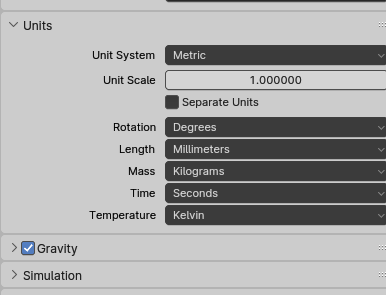
\includegraphics[width=12cm]{box/12}
        \end{center}

        Hrúbku obalu som zvolil podľa preglejky, ktorú som mal k dispozícii (4mm): \\

        \begin{center}
          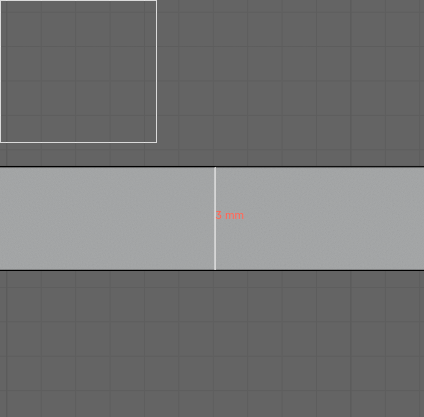
\includegraphics[width=12cm]{box/13}
        \end{center}

        Najprv som vytvoril kocku a pomocou rôznych nástrojov, ktoré nám Blender poskytuje, som vymodeloval spodnú časť obalu: \\

        \begin{center}
          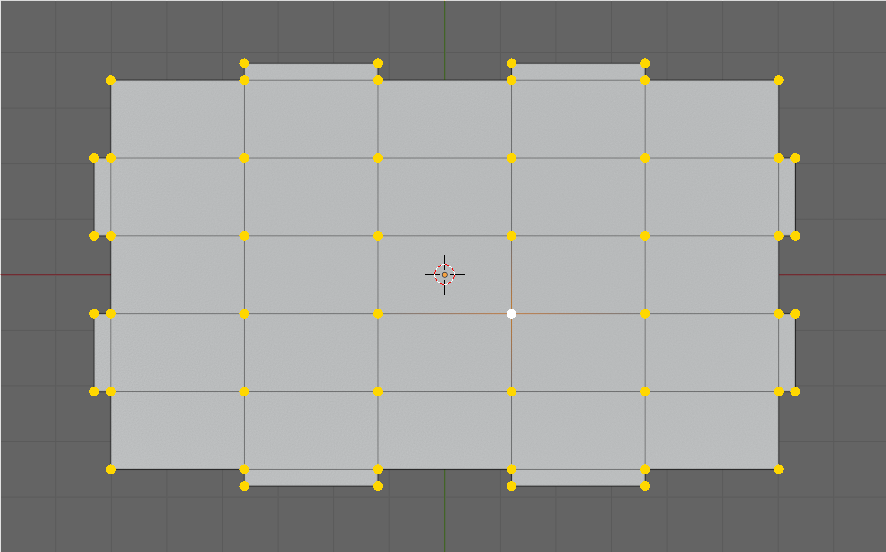
\includegraphics[width=12cm]{box/1}
        \end{center}

        Tak isto boli spravene bočné strany: \\

        Dlhsia strana: \\

        \begin{center}
          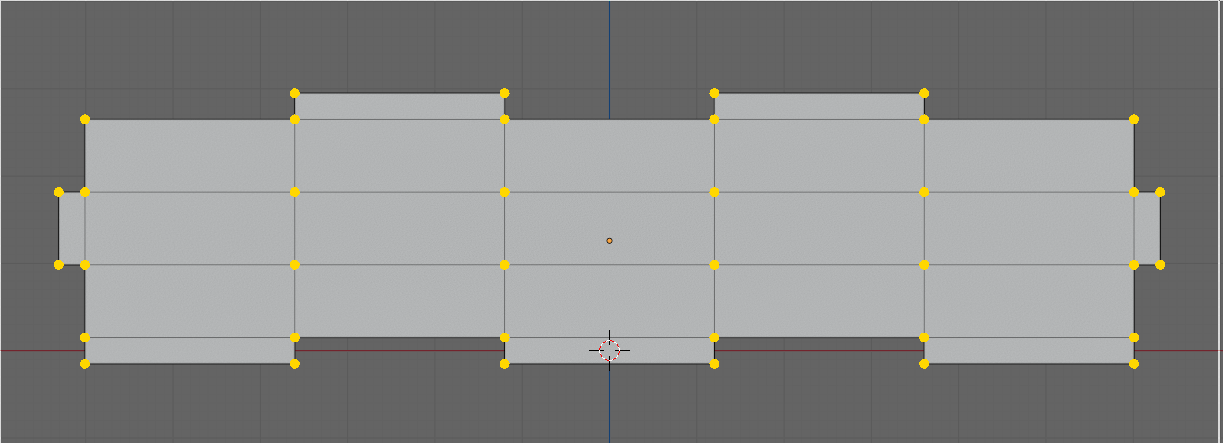
\includegraphics[width=12cm]{box/14} \\
        \end{center}

        Kratsia strana: \\

        \begin{center}
          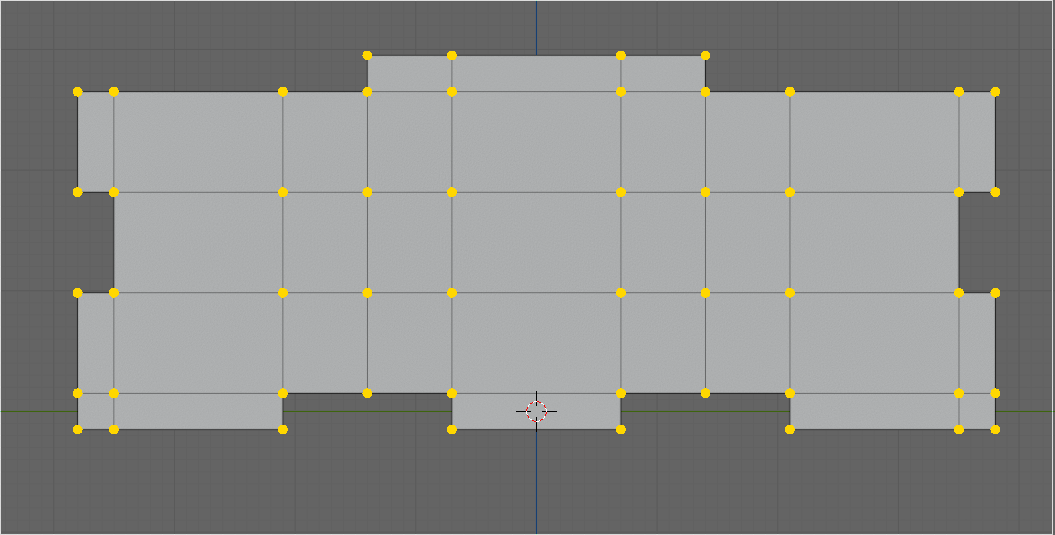
\includegraphics[width=12cm]{box/15}
        \end{center}

        Posledna horna cast modelu: \\

        \begin{center}
          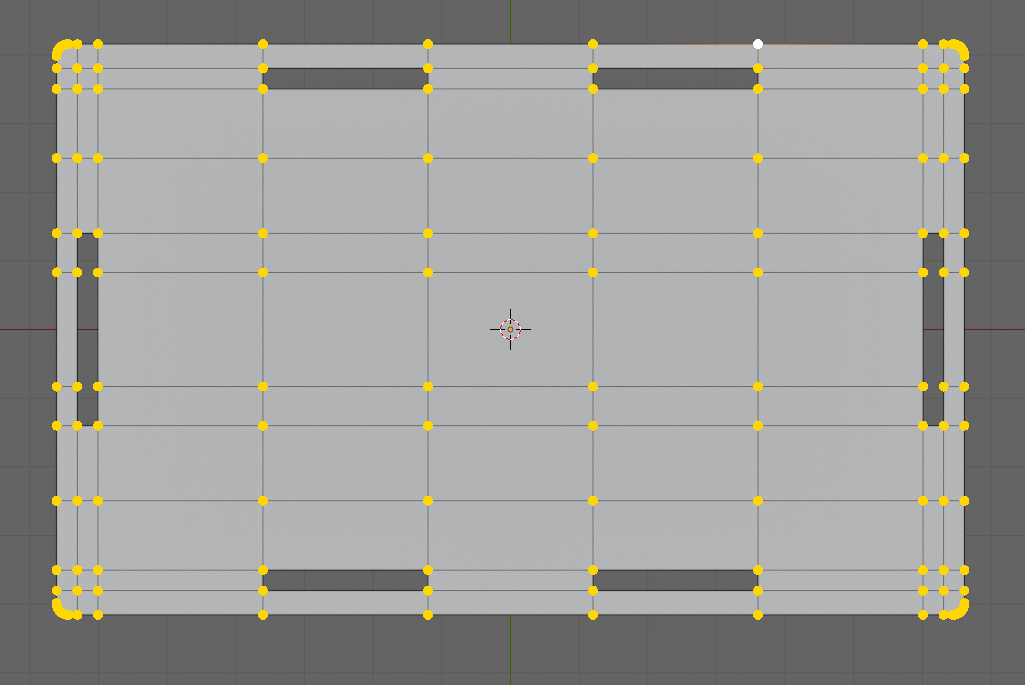
\includegraphics[width=12cm]{box/16}
        \end{center}

        Na konci som zaoblil hostre okraje obalu: \\

        \begin{center}
          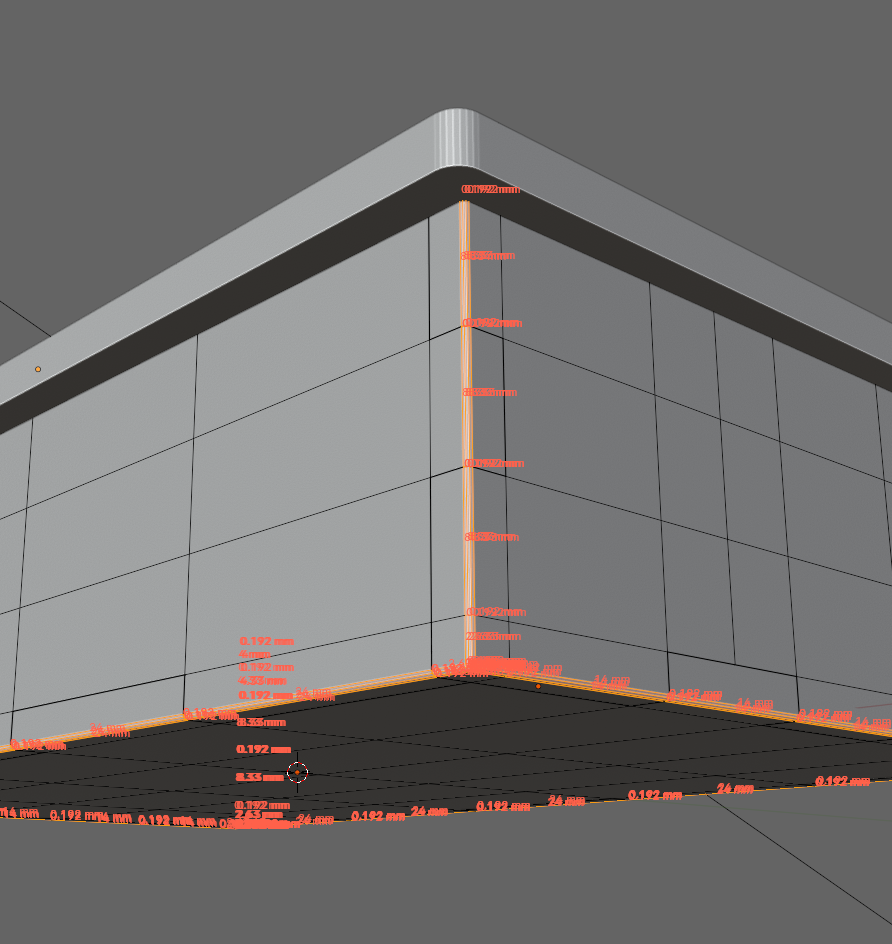
\includegraphics[width=12cm]{box/17}
        \end{center}

        3D vizualizácia hotoveho obalu: \\

        \begin{center}
          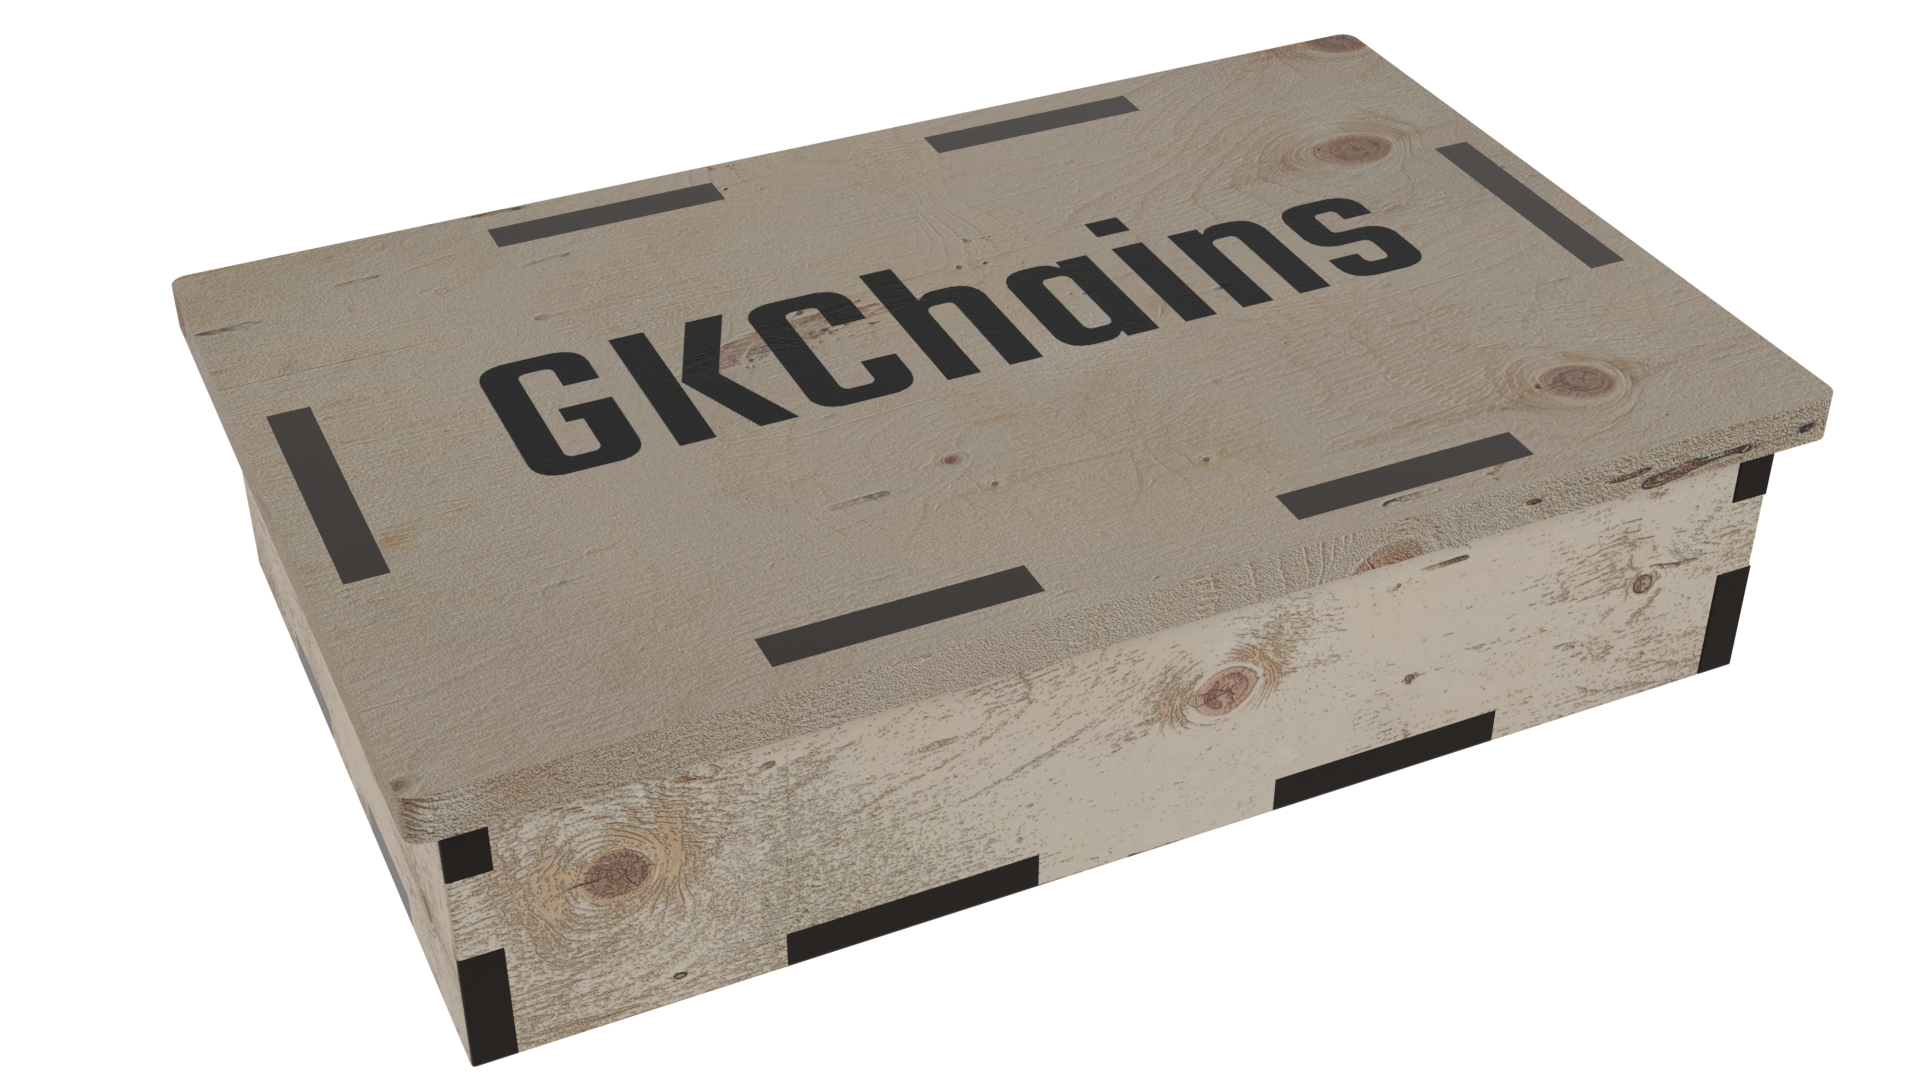
\includegraphics[width=14cm]{box/18}
        \end{center}

        Pre orezavanie materiálu som exportoval UV rozloženie každého dielu obalu do formátu .svg:

        \begin{center}
          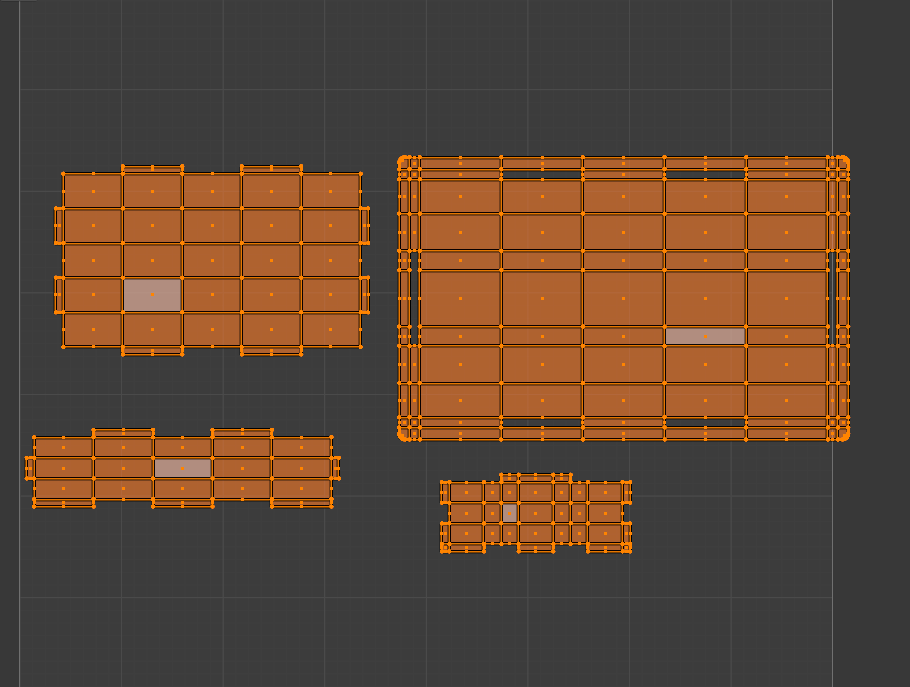
\includegraphics[width=14cm]{box/9}
        \end{center}

        A v aplikacie LightBurn som nastavil orezavanie a presne rozmery obalu:

        \begin{center}
          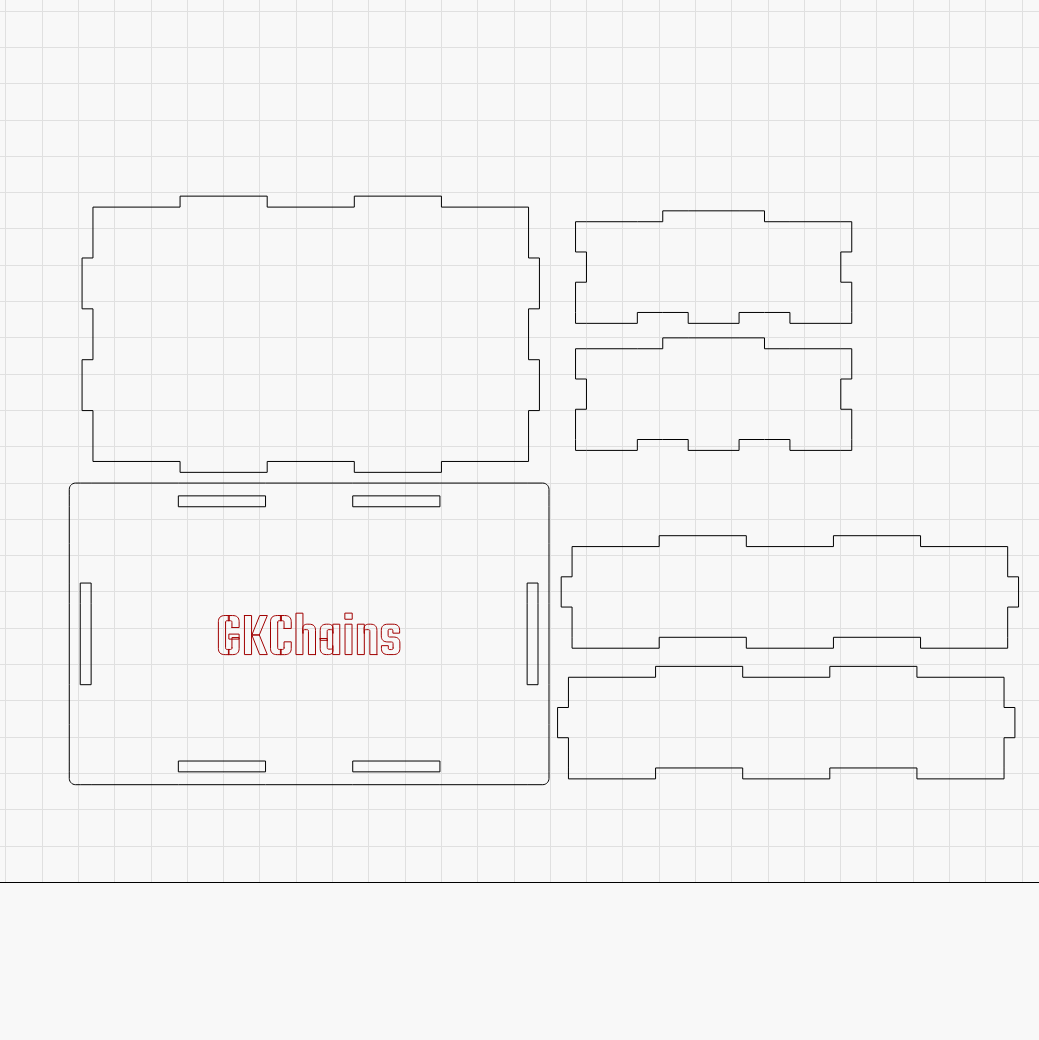
\includegraphics[width=14cm]{box/10}
        \end{center}

        Po vyrezaní obalov som ich zlepil špeciálnym PVA lepidlom pre drevo.

        PVA lepidlo (polyvinylacetát) je disperzia polyvinylacetátu vo vode s plastifikátorom a špeciálnymi prísadami. Má charakteristický slabý zápach. Používa sa na lepenie rôznych materiálov. Ako napríklad papier, drevo atď.

        \begin{center}
          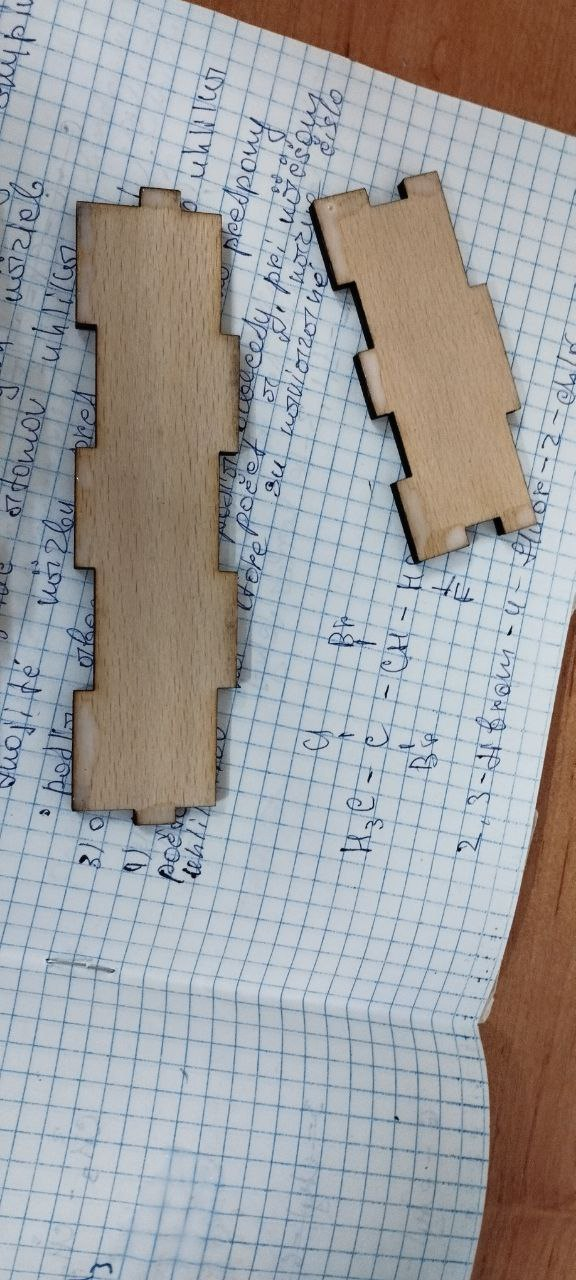
\includegraphics[height=14cm,angle=90]{box/19}
          \vfill{}
          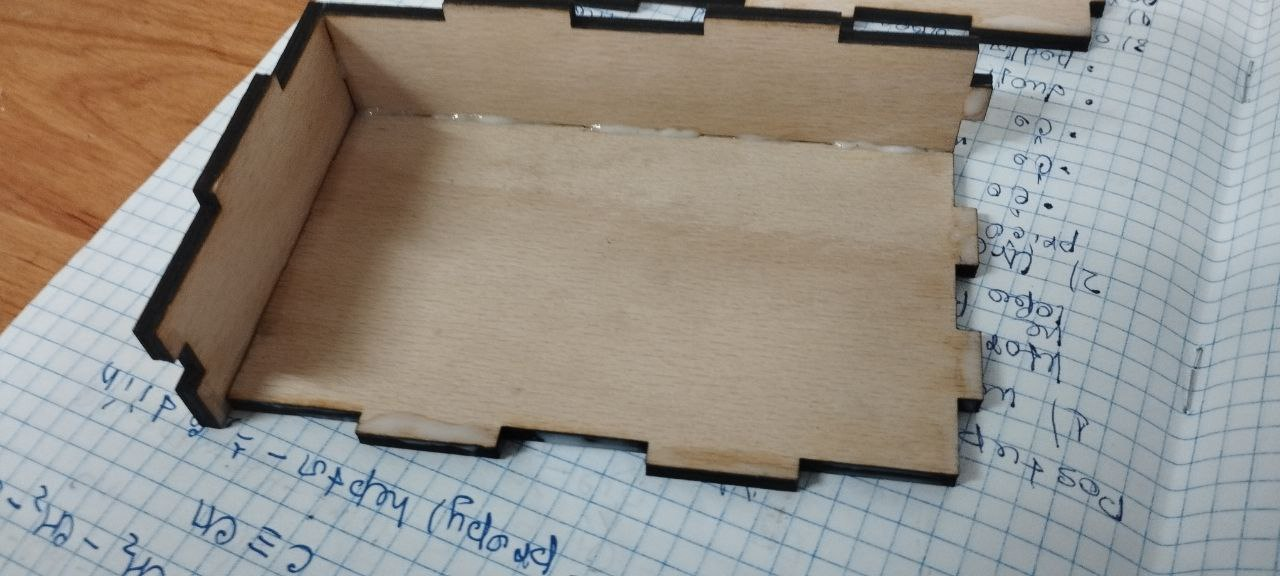
\includegraphics[width=14cm]{box/20}
        \end{center}

        Hotový obal vyzerá nasledovne:

        \begin{center}
          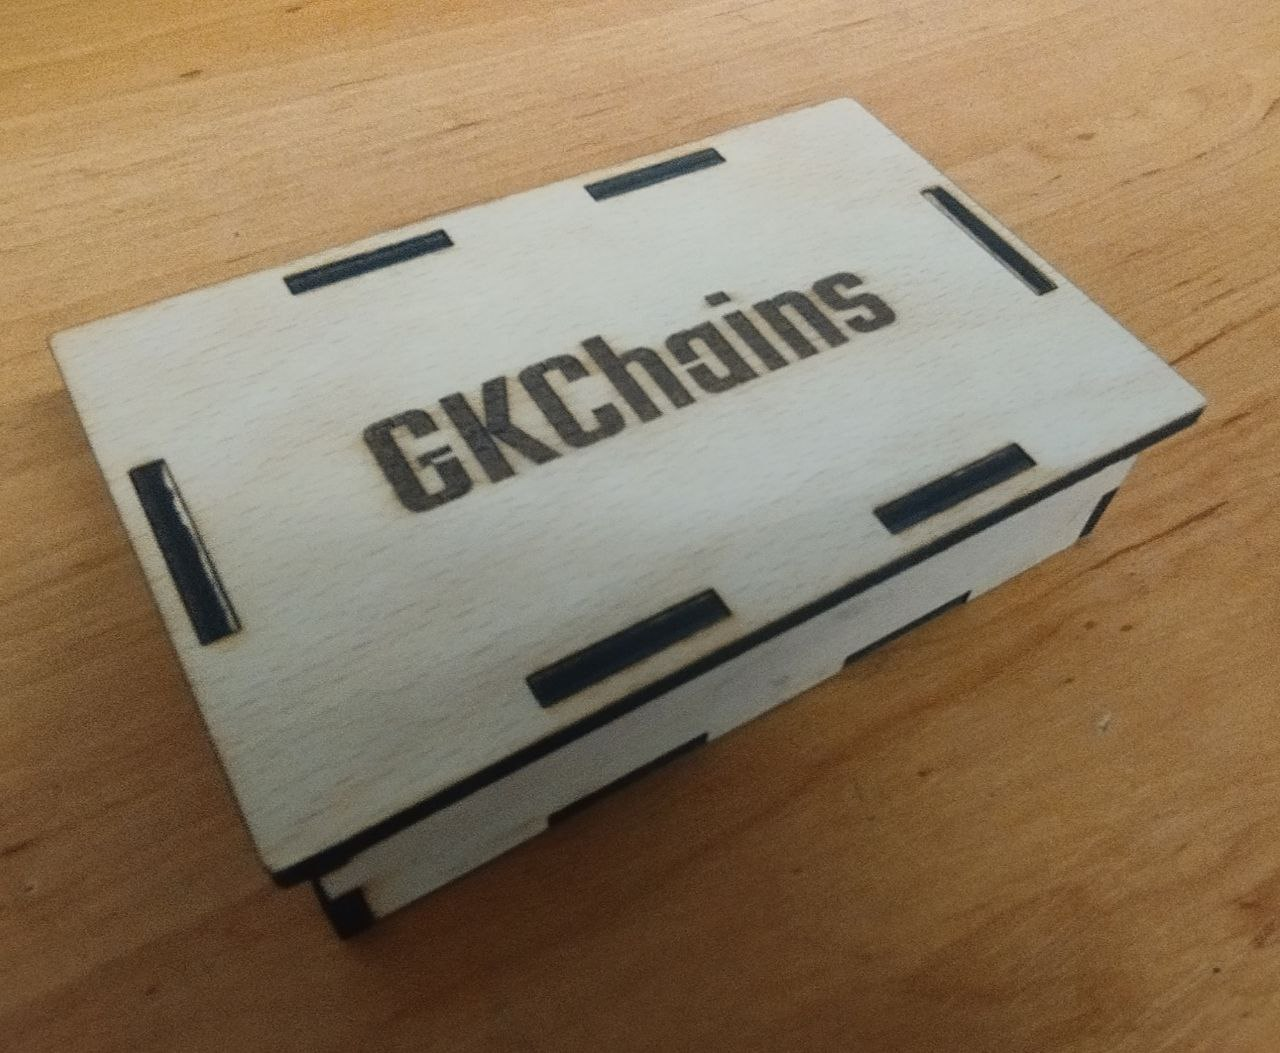
\includegraphics[width=14cm]{box/21}
        \end{center}
      \subsubsection{Kľučenieky}

      Kľúčenky modeloval som podľa nájdenej inšpirácie na pinterest.

      Príklad postupu modelovania kľúčenky:

      Rozdelil som objekt na par časti:

      \begin{center}
        
\includegraphics[width=10cm]{keychains/9}
      \end{center}

      Prvú časť, ktorú som smodeloval bola vyznačená bielym.

      Spravil som zakladnu formu:

      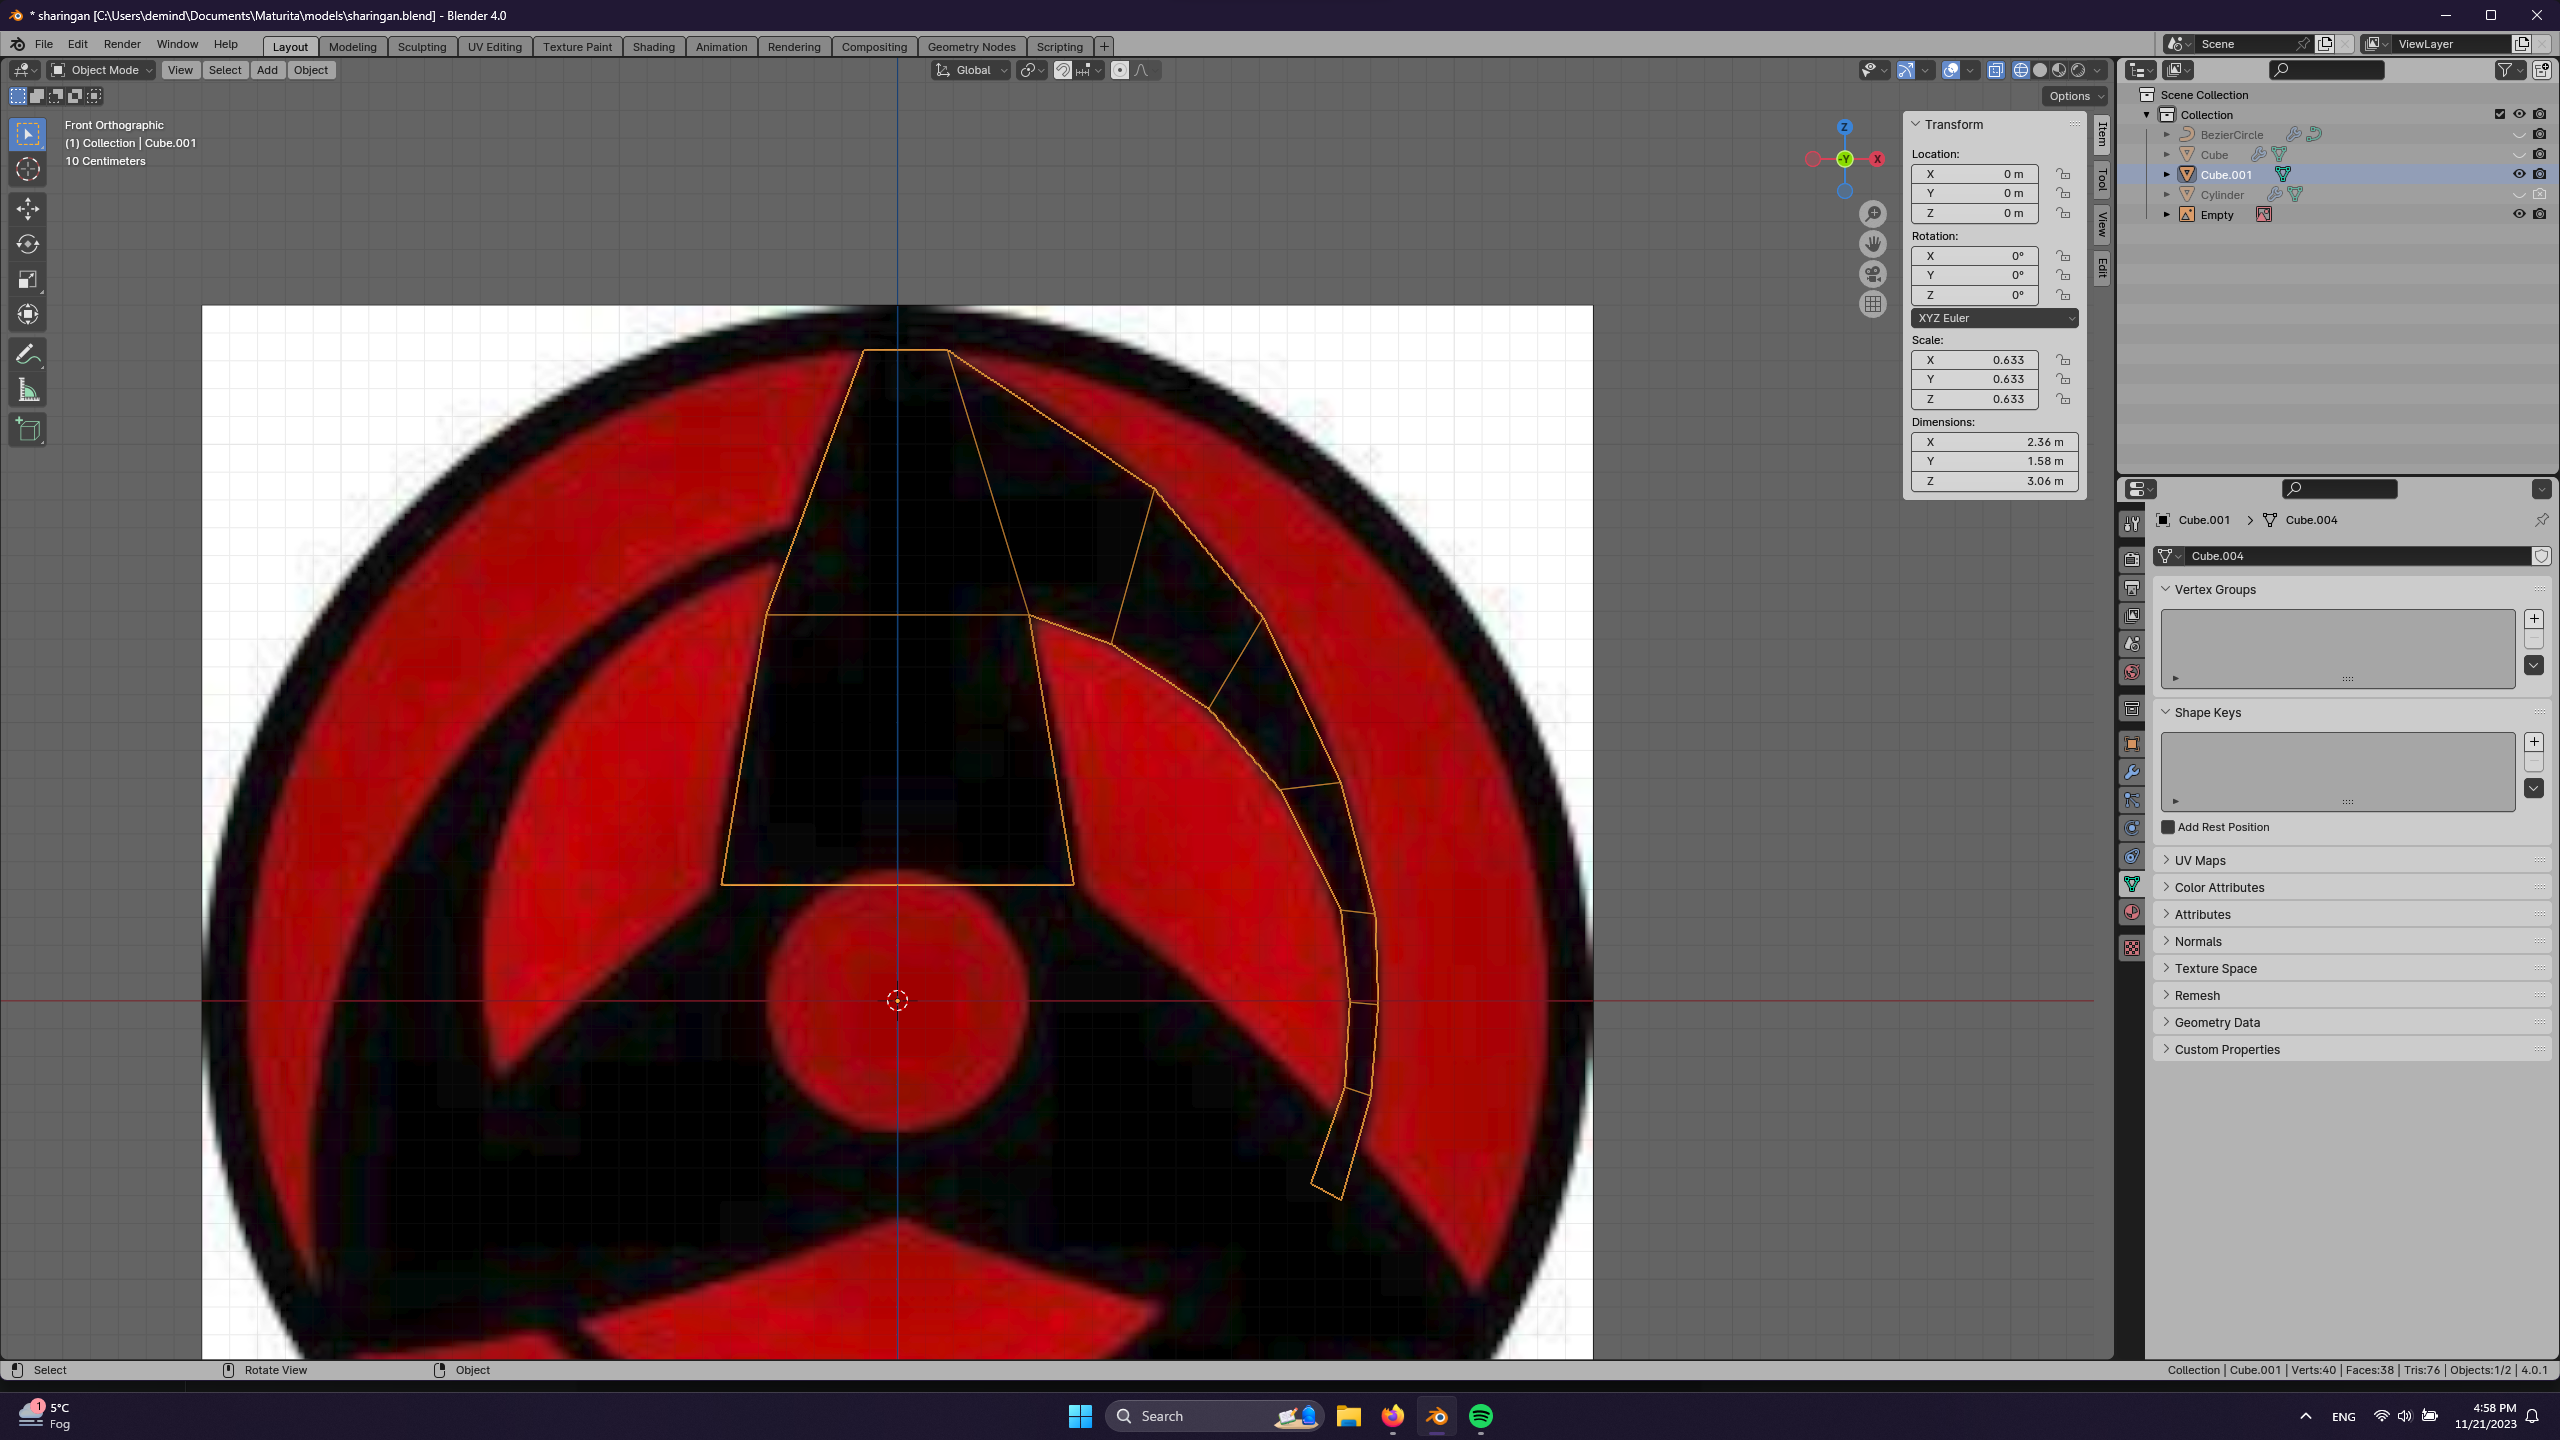
\includegraphics[width=14cm]{keychains/1}

      Pridal som strih na zväčšenie objemu v strednej časti modelu. \\

      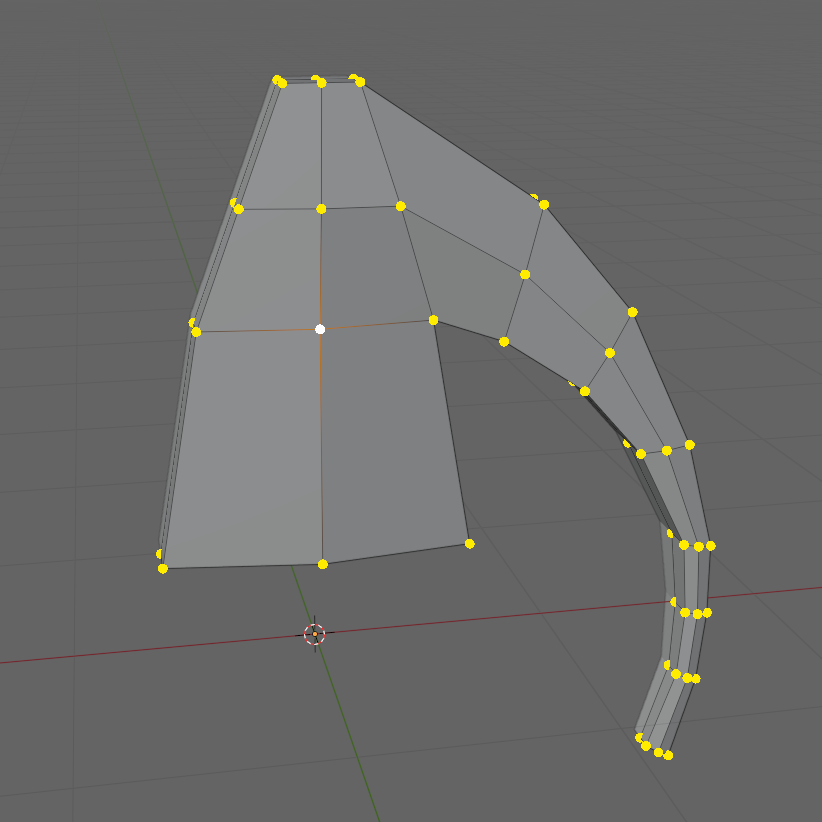
\includegraphics[width=14cm]{keychains/2}

      Objekt som vyhladil pomocou modifikátora Subdivision Surface na úrovni 2. Aktivoval som funkciu Smooth Shading (Hladké tieňovanie), aby som dosiahol efekt vyhladenia objektu: \\

      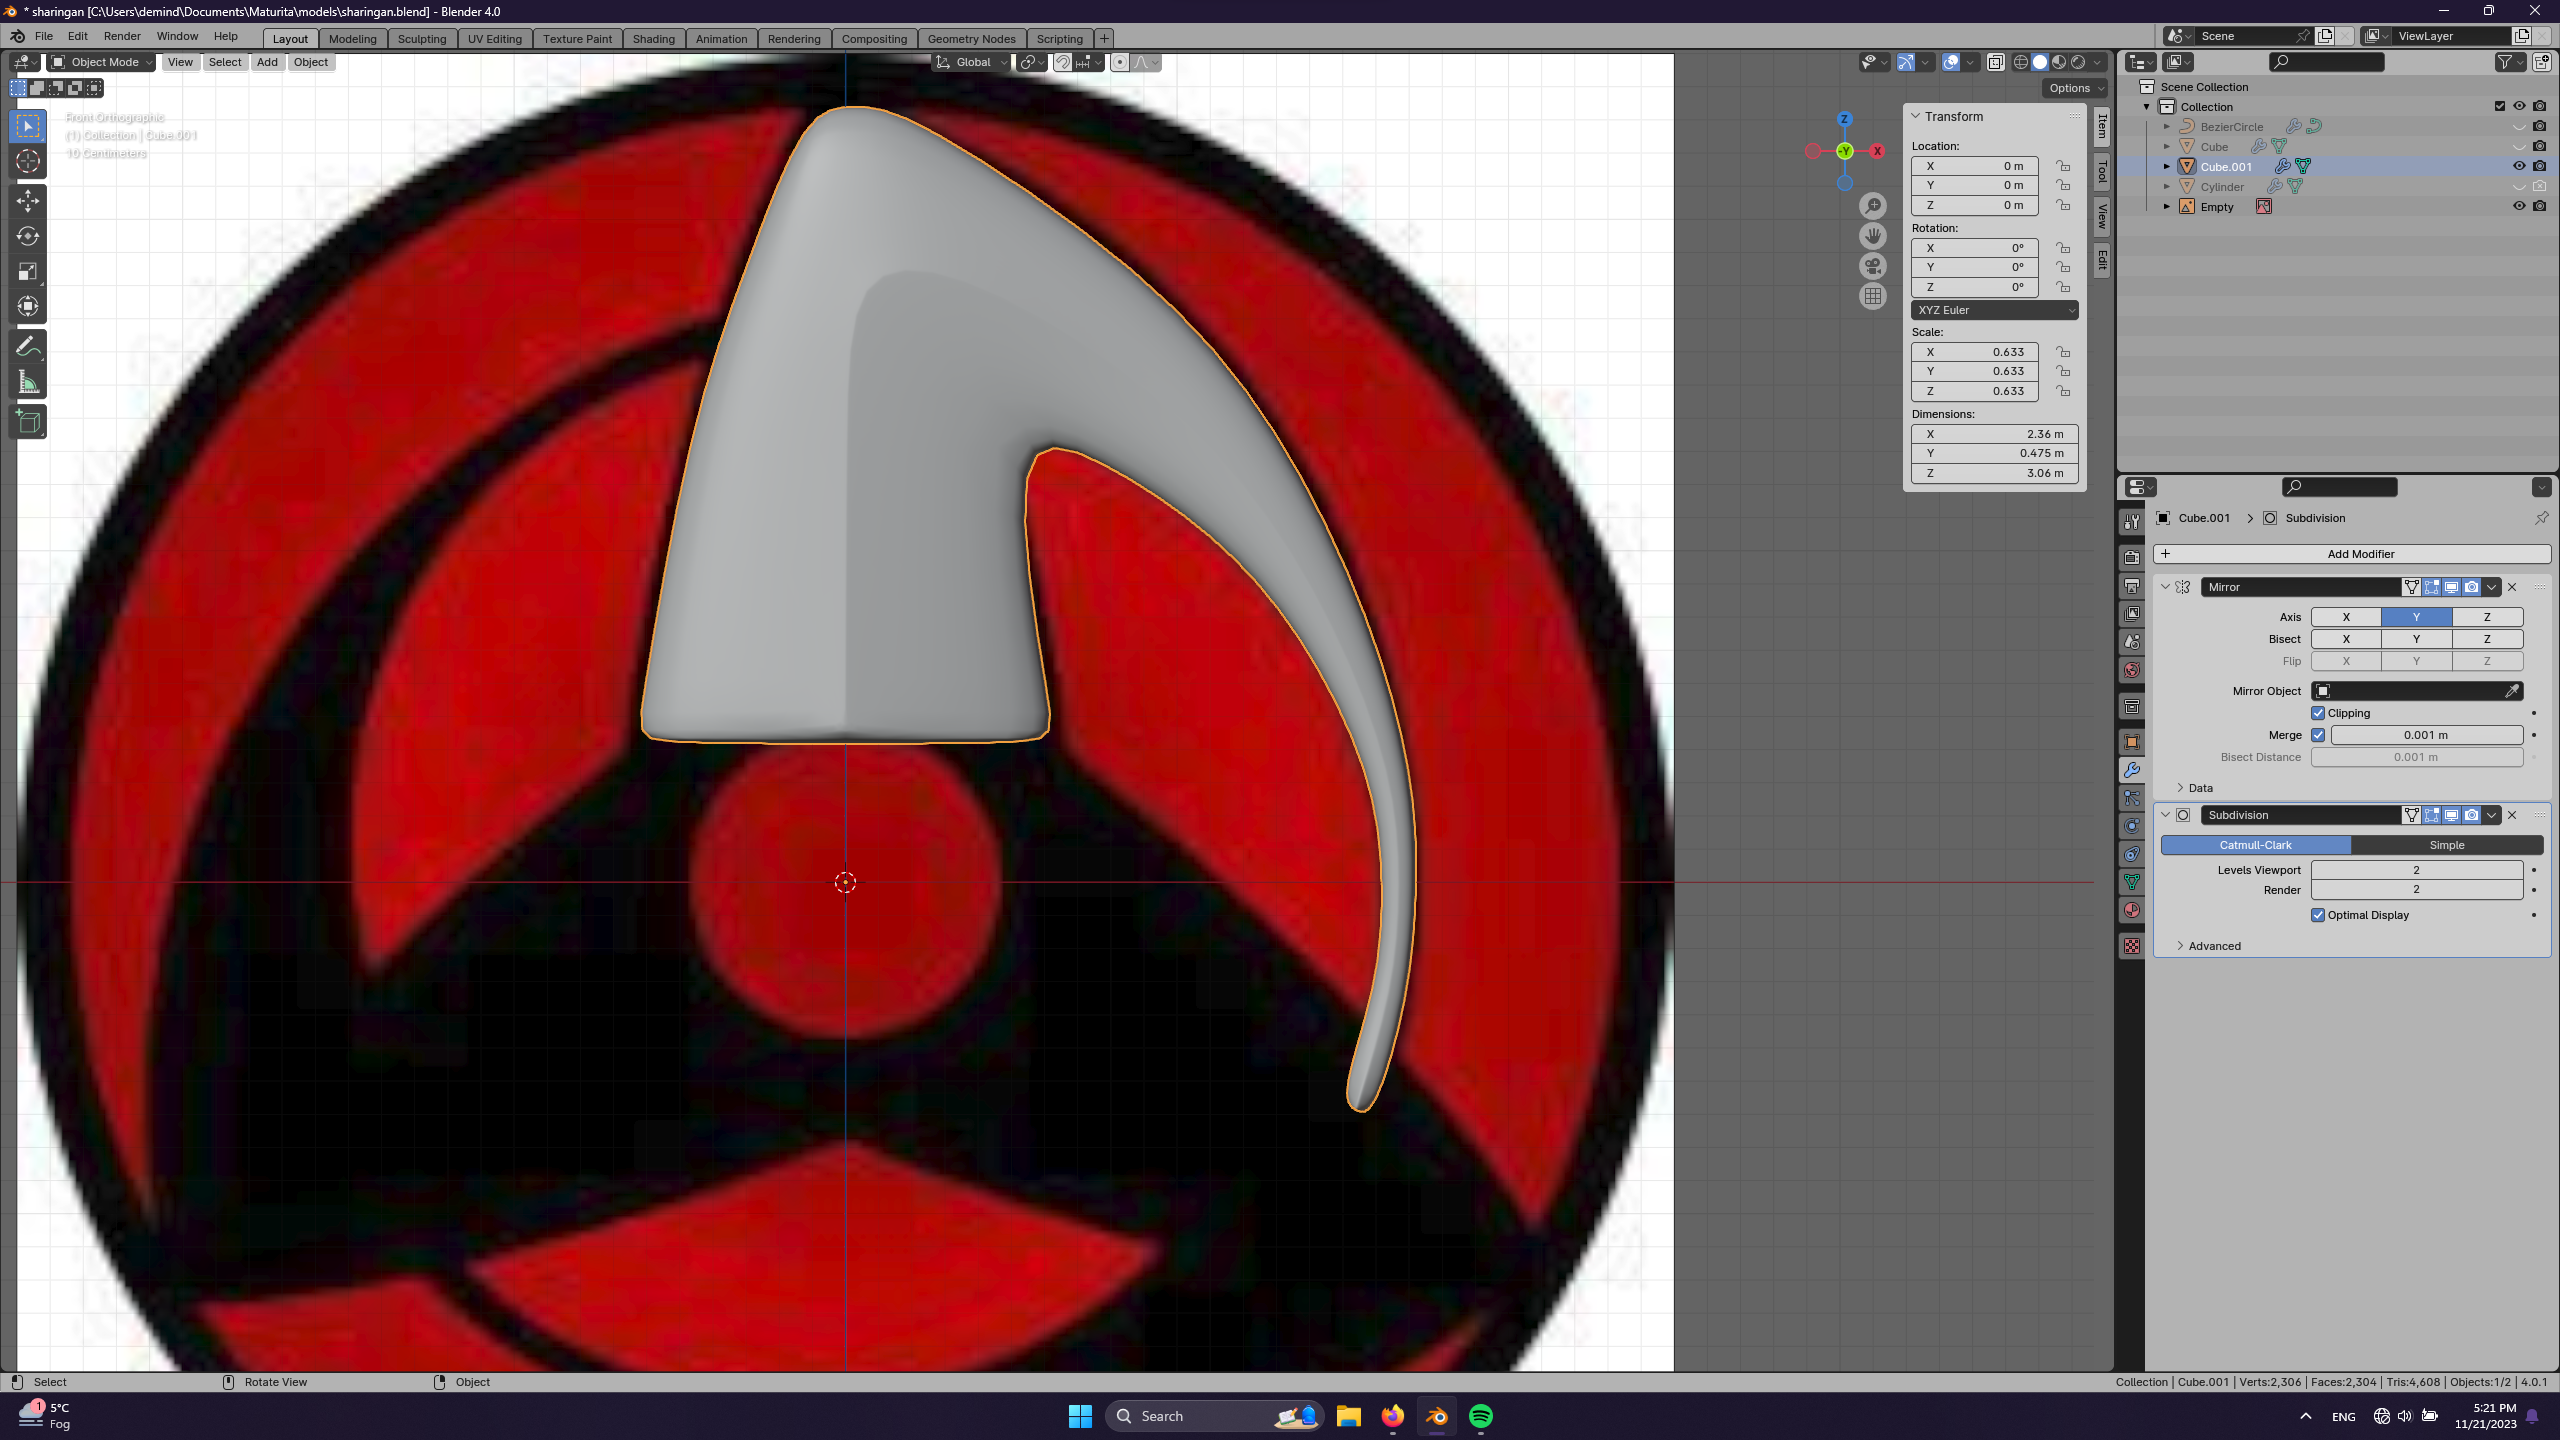
\includegraphics[width=14cm]{keychains/4}

      Objekt som skopíroval 2-krát a otočil ho tak, ako je znázornené: \\

      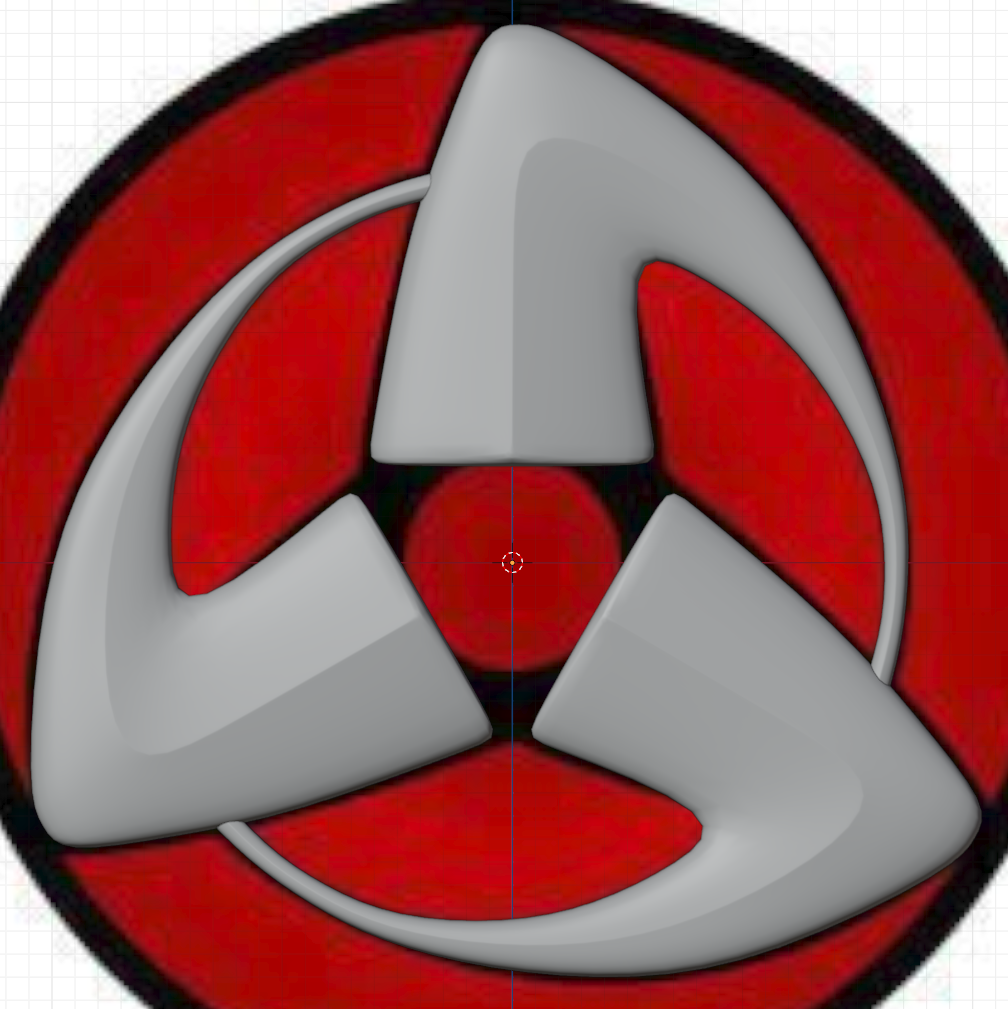
\includegraphics[width=14cm]{keychains/5}

      Všetky tri objekty som spojila do jedného. \\

      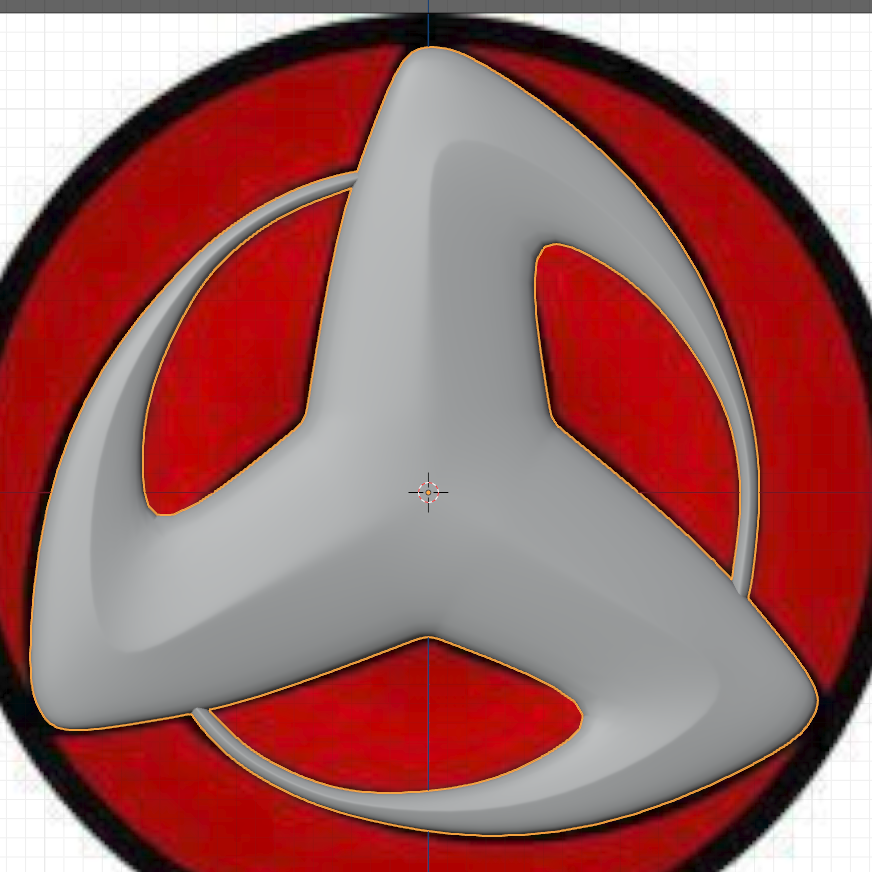
\includegraphics[width=14cm]{keychains/6}

      \newpage
      Potom som v strede objektu vyrezal dieru pomocou modifikátora Boolean. Pidal som poslednu čast modelu: \\

      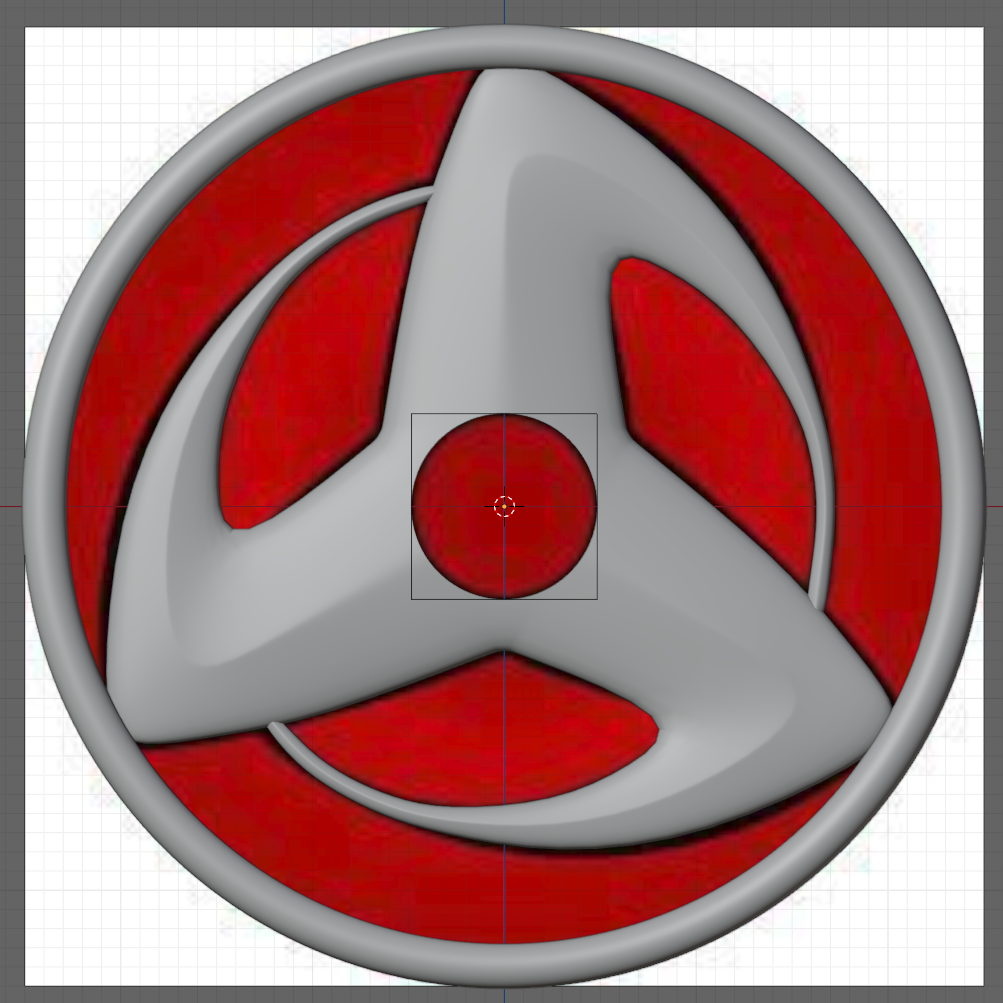
\includegraphics[width=14cm]{keychains/7}

      Na záver som pridal kruh, ktorý drží kľúčenku na kľúčoch: \\

      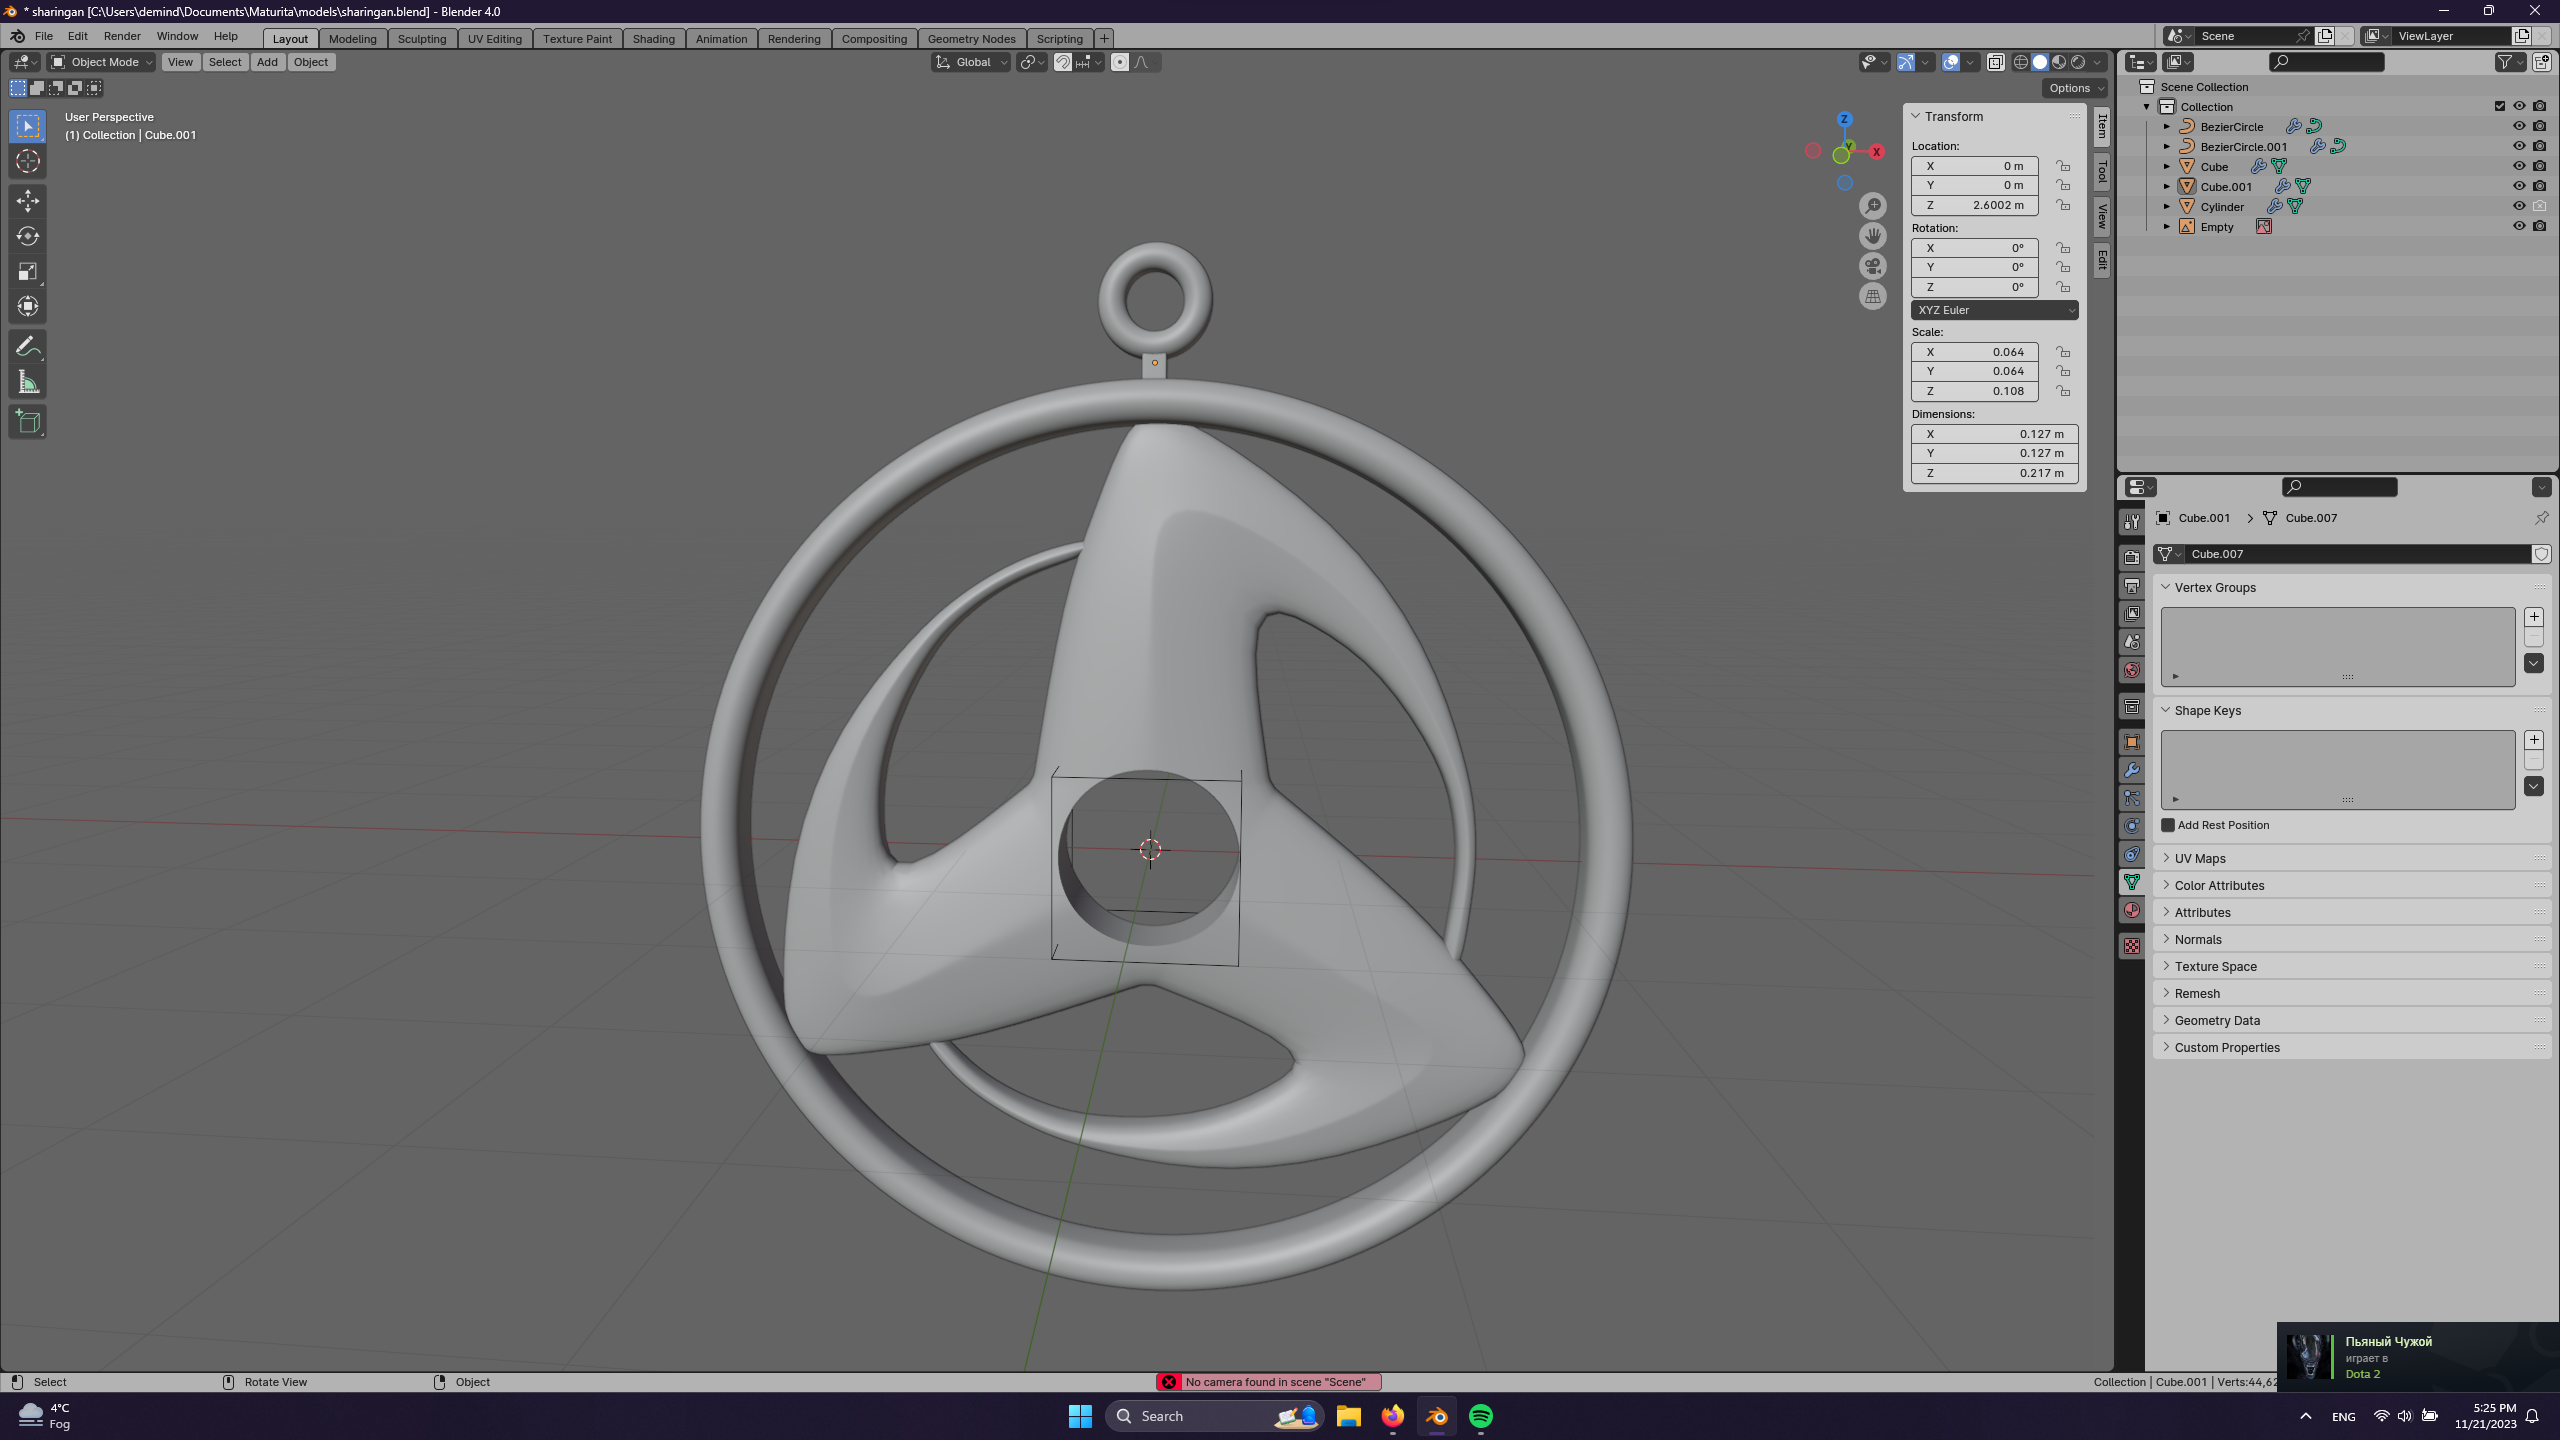
\includegraphics[width=14cm]{keychains/8}

      \newpage
      Render kľúčenky: \\

      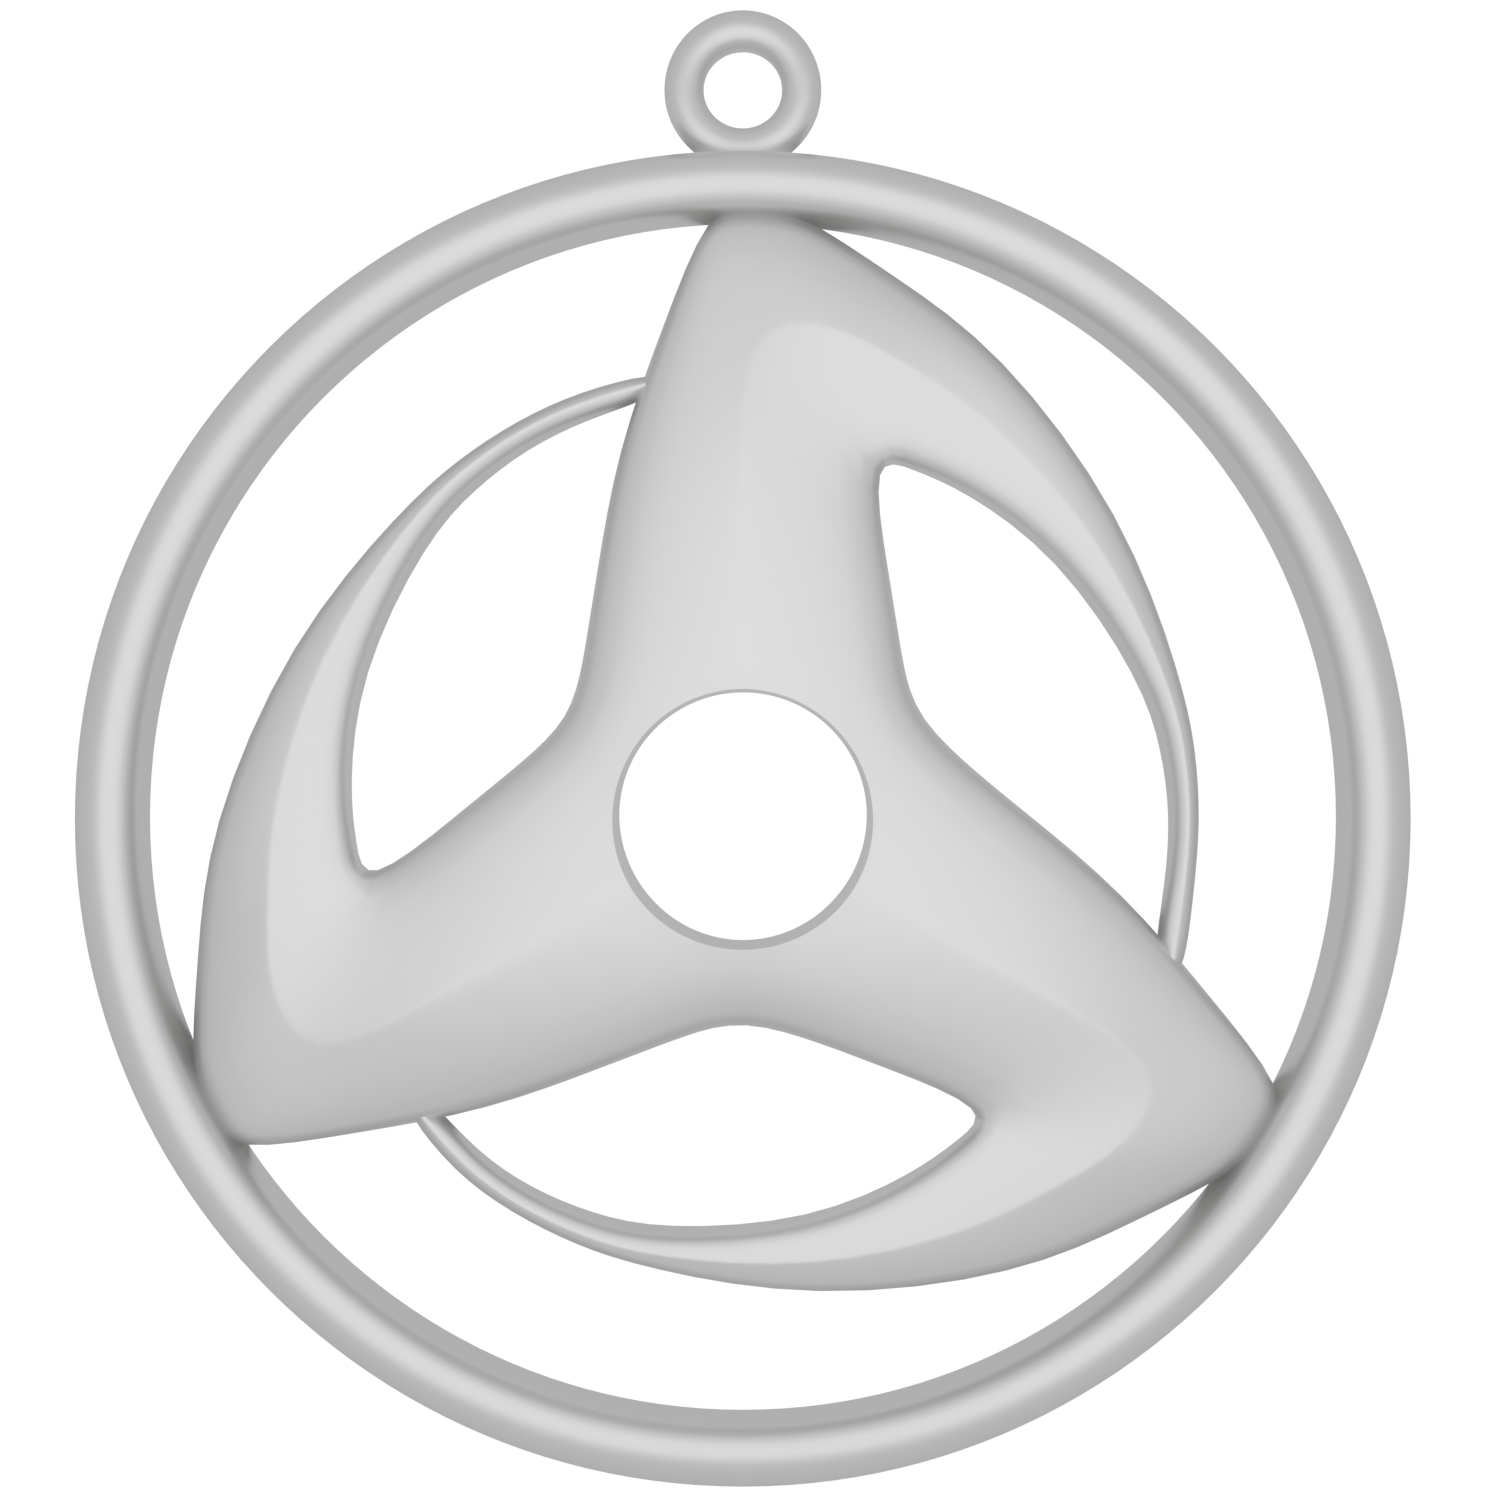
\includegraphics[width=14cm]{keychains/10}

      \subsubsection{Web stranka}

  \section{Cenova kalkulacia}

  \section{Zaver}

  \section{Zoznam použitej literatúry}
\end{document}

% https://wiki.archlinux.org/title/Neovim
% https://cs.puntomarinero.com/pva-glue-composition-and-characteristics/
% https://habr.com/ru/companies/lpcloud/articles/236439/
